\chapter{Architettura a Microservizi}

Un'architettura a microservizi è una variante dell'architettura \textit{Service oriented} che prevede di strutturare un'applicazione come un insieme di moduli disaccoppiati tra loro, indipendentemente rilasciabili, manutenibili e testabili.\\
I servizi possono comunicare tra loro tramite protocolli di vario tipo, sia sincroni che asincroni.

\section{Scalabilità}
Un'applicazione enterprise nasce naturalmente come costituita da un singolo blocco in esecuzione su di un dispositivo (fisico o virtuale).\\
I sistemi di questo tipo hanno successo quando, una volta rilasciato il software, il numero di utilizzatori rimane limitato e la manutenzione non introduce troppe nuove funzionalità.
Altrimenti, per evitare un deterioramento delle performance o eventuali fallimenti, è necessario affrontare il tema della scalabilità quando il sistema è già online, nel caso questo non sia già stato fatto in fase di progettazione.

\subsection{The Scale Cube}
In figura \ref{fig:scale-cube}\cite{the_art_of_scalability} è mostrato uno dei possibili modelli su cui è possibile lavorare per ottenere un'applicazione scalabile.
In questa rappresentazione è possibile muoversi lungo i tre assi cartesiani per ottenere diversi benefici:

\begin{figure}[h]
	\centering
	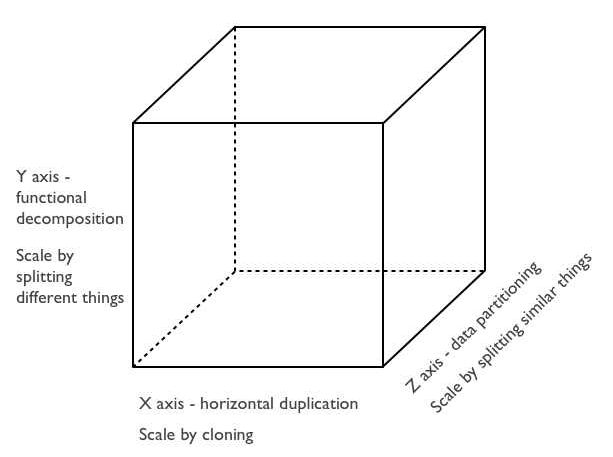
\includegraphics[scale=0.5]{img/scale-cube}
	\caption{Modulo ad architettura ports and adapters}
	\label{fig:scale-cube}
\end{figure}


\subsubsection{Asse X}
Scalare un sistema \textit{sull'asse X} significa avere più repliche della stessa applicazione in produzione.
Questo permette di gestire un maggior numero di richieste al secondo, eliminare i \textit{single point of failure} e non richiede grandi costi aggiuntivi di progettazione o rifattorizzazione.
Gli accessi sono gestiti da un \textit{load balancer} che avrà la responsabilità di inoltrare una richiesta all'istanza più appropriata in base a vari criteri, quali zona geografica, presenza di guasti, carico di lavoro ecc...
La scelta di quest'ultimo componente è piuttosto libera: è sufficiente un sistema che opera su un livello basso come rete o trasporto, in quanto non è necessario accedere ai dati applicativi.\\
Ogni nodo potenzialmente può avere a che fare con tutte le informazioni gestite dall'applicazione, quindi questo tipo di organizzazione non migliora i requisiti di memoria per istanza.

\subsubsection{Asse Z}
Scalare un sistema \textit{sull'asse Z} significa avere lo stesso codice replicato su più server come nel caso precedente, ma stavolta ogni copia è responsabile di un sottoinsieme dei dati: il load balancer dovrà quindi inoltrare le richieste in base al contenuto di esse, e dovrà probabilmente operare a livello applicazione.\\
Questa scelta permette di ridurre le risorse necessarie ad ogni istanza, compresa la quantità di storage o di memoria riservata alla cache.

\subsubsection{Asse Y}
Scalare un sistema \textit{sull'asse Y} significa effettuare una partizione del software per tipi di dati e/o funzionalità, partendo da un'analisi dei casi d'uso e modello di dominio.\\
Si ottengono così più istanze uniche, ognuna con le proprie responsabilità.
La complessità del software viene quindi ridotta, le risorse ottimizzate e la manutenibilità migliorata.\\
Questo approccio incide maggiormente sulla fase di progettazione, anche se un modo rapido per implementare questa strategia su un sistema preesistente può essere quello di replicare l'applicazione per intero come nei casi precedenti e delegare ad ogni replica un particolare compito sulla base delle divisioni individuate per mezzo di un load balancer di livello applicazione.

\section{Partizionamento in microservizi}
Progettare un sistema a microservizi non è semplice quanto progettarne uno monolitico o service oriented tradizionale: difficilmente infatti un software verrà pensato già partizionato, e a causa delle diverse complessità che questo approccio si porta dietro non è consigliabile utilizzarlo come prima carta.\\
Solitamente si sceglie di passare a tale architettura in un secondo momento, per esempio dopo molti interventi di manutenzione, quando il codice inizia ad essere troppo ampio e complesso.\cite{microservices_architecture}
In termini di \textit{Scale Cube} il partizionamento in microservizi agisce sull'asse Y.

Avere una serie di componenti di dimensione più ridotta produce molti vantaggi, tra i quali:
\begin{itemize}
	\item Maggiore manutenibilità e facilità di testing.
	\item Maggiore indipendenza e minor dimensione dei team di lavoro.
	\item Migliore isolamento dei guasti.
\end{itemize}

Ogni servizio inoltre:
\begin{itemize}
	\item Può essere scalato in modo indipendente.
	\item Può essere rilasciato in modo indipendente.
	\item Può avere il proprio stack tecnologico.
	\item Può ottenere risorse in modo mirato.
\end{itemize}

Vi sono naturalmente anche svantaggi nell'adottare questo tipo di architettura, per esempio:
\begin{itemize}
	\item Non è semplice trovare il giusto set di servizi: Il rischio è di ottenere come risultato un \textit{monolite distribuito}, ovvero un set di servizi accoppiati tra loro che necessitano di evolvere ed essere rilasciati contemporaneamente.
	Vengono in questo modo sommati gli svantaggi delle architetture monolitica e a microservizi.
	\item Ideare un sistema distribuito è un'operazione complessa: Meccanismi come lo scambio messaggi, le transazioni e le query diventano più complessi.
	\item Aggiungere funzionalità che necessitano l'aggiornamento di più servizi è più complesso: Sarà necessario un piano di aggiornamento che tenga conto delle dipendenze tra moduli.
\end{itemize}

\section{Scambio di messaggi}
//ASINCRONO VS SINCRONO

\section{Gestione delle transazioni}
Una transazione di business in un sistema monolitico corrisponde spesso con una transazione locale che inizia all'arrivo della richiesta e termina all'invio della risposta.\\
A meno che una funzionalità non richieda l'intervento di un solo modulo, in un sistema a microservizi questo non è possibile, in quanto le transazioni sono locali al singolo servizio.

Si prenda come esempio la figura \ref{fig:mono-transaction}: in questo caso l'utente interagisce con un sistema monolitico facendo richiesta di un servizio che necessita di effettuare tre operazioni sul database.
Una transazione locale viene avviata in corrispondenza della prima azione e chiusa dopo la terza.
Nel caso vi sia un errore durante la processazione un rollback riporterà il sistema in uno stato consistente.

\begin{figure}[h]
	\centering
	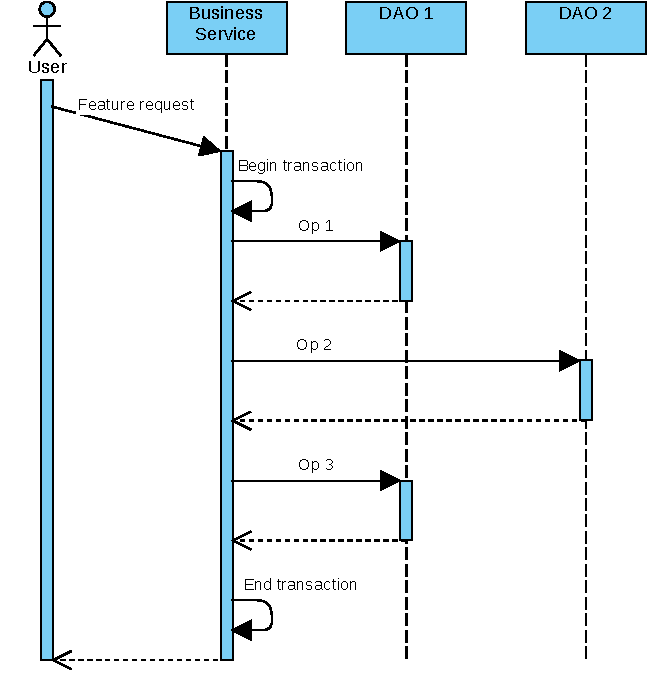
\includegraphics[width=\textwidth]{img/monolithic-transaction}
	\caption{Gestione di una transazione in un sistema monolitico}
	\label{fig:mono-transaction}
\end{figure}

Ipotizziamo che la stessa funzionalità sia richiesta ad un sistema con architettura a microservizi e che i componenti coinvolti siano due.
In questo caso verrà aperta una transazione per servizio, e in caso di successo lato utente non vi sarà nessuna differenza (vedi figura \ref{fig:micro-transaction-err}).\\
In questo scenario però sorgono alcuni problemi, ovvero:
\begin{itemize}
	\item La transazione sul primo servizio rimane aperta per tutta la durata della seconda operazione che è delegata ad un sistema esterno.
	\item Nel caso vi sia un errore sulla terza operazione si avrebbe un'inconsistenza, in quanto la transazione del servizio 1 sarebbe annullata, ma non quella del servizio 2, ormai terminata.
	\item Le comunicazioni sincrone tra servizi sono sconsigliate.
\end{itemize}

\begin{figure}[h]
	\centering
	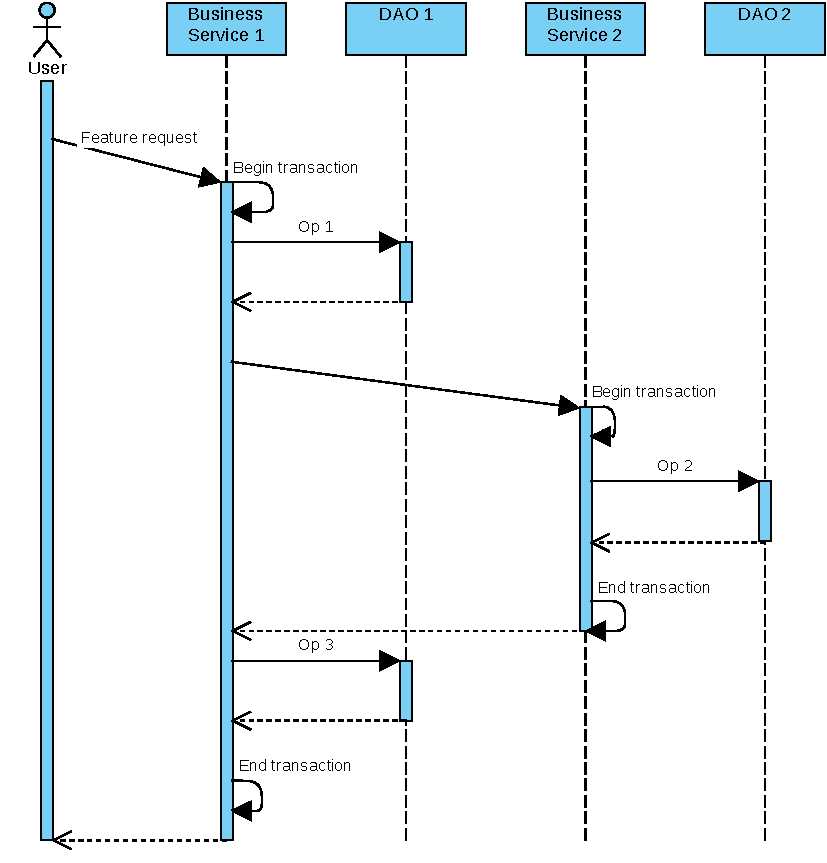
\includegraphics[width=\textwidth]{img/microservices-transaction-error}
	\caption{Cattiva gestione di una transazione in un sistema a microservizi}
	\label{fig:micro-transaction-err}
\end{figure}

Un approccio migliore, che cerca di disaccoppiare al meglio i servizi è quello riportato in figura \ref{fig:micro-transaction}.
I punti salienti sono:
\begin{itemize}
	\item Sono state introdotte comunicazioni asincrone
	\item \'E stato introdotto un sistema di notifica (approfondito in seguito) per notificare la terminazione di un servizio.
	\item Il primo servizio adesso effettua necessariamente due transazioni, anche per la natura asincrona dello scambio messaggi.
\end{itemize}

\begin{figure}[h]
	\centering
	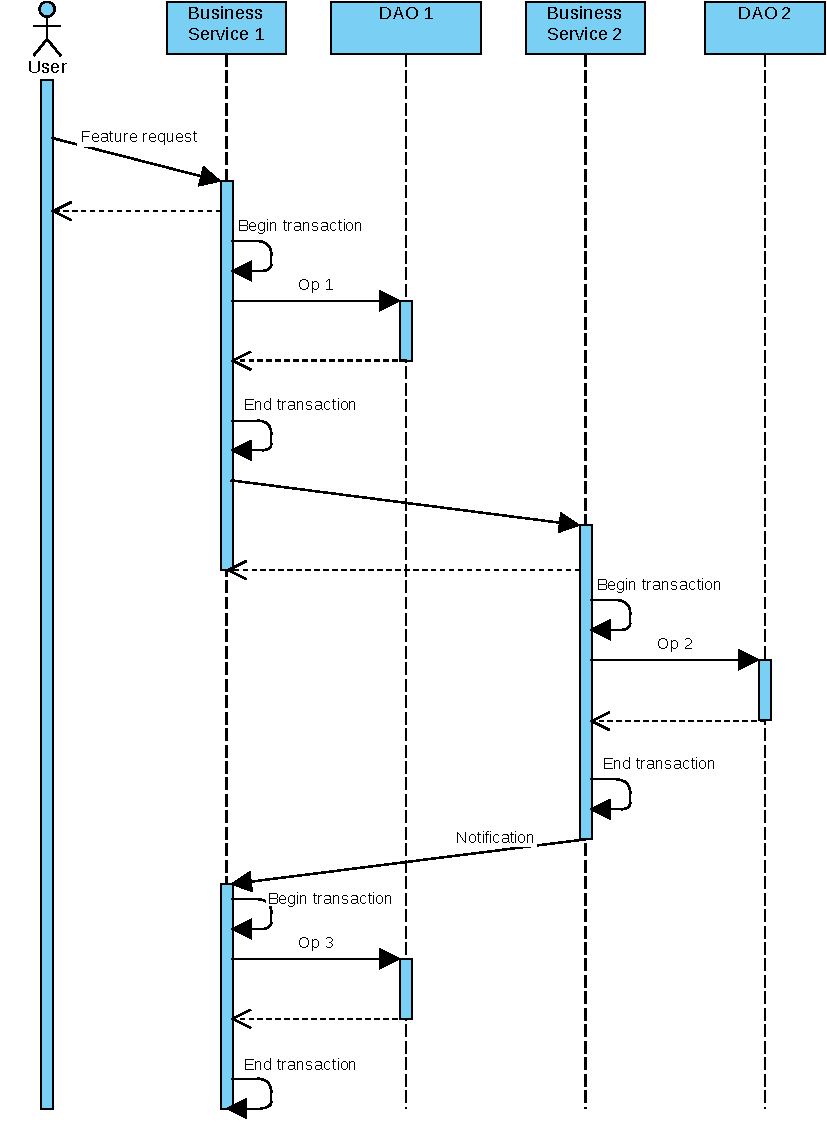
\includegraphics[width=\textwidth]{img/microservices-transaction}
	\caption{Gestione di una transazione in un sistema a microservizi}
	\label{fig:micro-transaction}
\end{figure}

https://microservices.io/patterns/data/saga.html

Con il termine \textit{saga} si intende un insieme di piccole transazioni locali autoconsistenti.\\
Il coordinamento avviene in modo distribuito: ogni servizio lancerà eventi in caso di completamento o fallimento di una transazione; questi saranno quindi interpretati dagli altri moduli.\\
\'E possibile delegare le opzioni di coordinamento ad oggetti appositi.

\section{Caratteristiche di un microservizio}

Temi ricorrenti quando si parla di microservizi sono quelli riguardanti la dimensione che un servizio deve avere, il numero di responsabilità, l'integrità delle informazioni ecc...\\
La linea guida principale da seguire è quella di fare in modo che i servizi siano il più possibile indipendenti tra loro, favorendo coesione, evitando un eccessivo accoppiamento.\\
Un servizio per essere tale dev'essere rilasciabile in modo indipendente dagli altri: esso infatti è l'unità minima dell'architettura. Ognuno può potenzialmente utilizzare la propria tecnologia, cosa che favorisce l'evoluzione ed evita che il software nel tempo resti legato ad una tecnologia datata.\\
Il partizionamento del monolite deve portare ad avere un certo numero di servizi disaccoppiati ma coesi: occorre studiare bene quali siano i giusti confini lungo cui tagliare il software, in modo che i nodi possano lavorare in indipendenza, ognuno con le proprie responsabilità.